%\chapter{sciencetech}

%%%%%%%%%%%%%%%%%%%%%%%%%%%%%%%%%%%%%%%%%%%%%%
\section{Charged particle beam studies}
Science description


One of the crucial goal of the protoDUNE-SP experiment is to measure and study the response of the detector to charged
particles of different types and energies. Results from these measurements serve to
assess systematic detector uncertainties and validate MC simulations. They also enable
validation and tuning of event reconstruction algorithms and particle identification tools.

The beam-line will produce particles with properties partially covering the 

\begin{cdrfigure}[Placeholder ]{ParticleMomenta}{Placeholder: Left: Momenta distributions of particles produced by the neutrinos from DUNE neutrino beam. Right: the predicted rate of particles as a fuction of therir momentum for the charged particle beam-line.}
  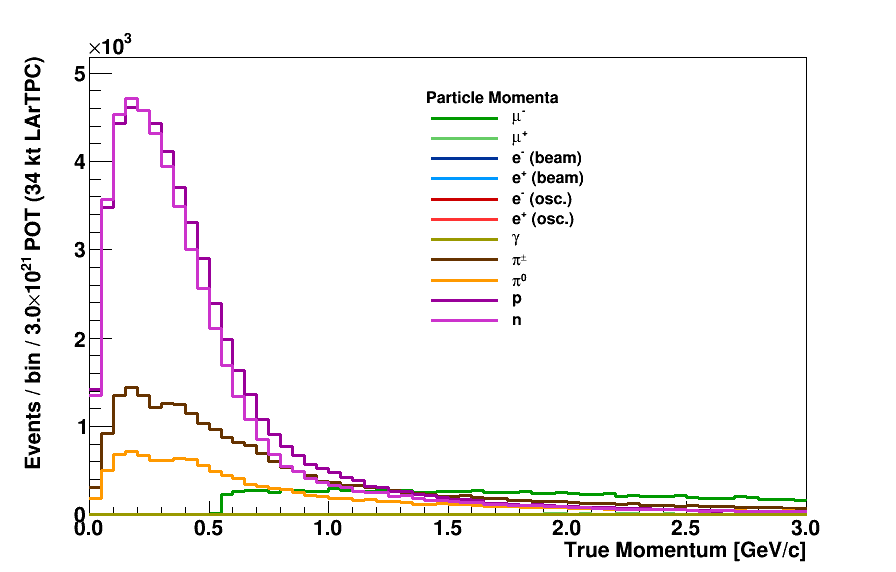
\includegraphics[width=0.8\textwidth]{figures/Momenta_per_Particle}
\end{cdrfigure}

The main studies that will be performed using charged particles from the beam and particles created by cosmic muons are
(Each of the point below will be described in details in the next draft.)
\begin{itemize}
\item Characterisation of  hadronic showers (high momenta) and  topologies of the hadronic interactions (low momenta).
\item Characterisation of electromagnetic showers.
\item Study $e/\gamma$ separation capabilities.
\item Measurement of the field distortion effect (space-charge, LAr flow, beam window effect, etc).
\item Measure event reconstruction efficiencies as a function of energy and particle type
\item Measure performance of particle identification algorithms as function of energy
\item Validate accuracy of Monte Carlo simulations for relevant energy ranges as well as
directions with respect to the wire-plane geometry
\end{itemize}


Additional items to be described in this section
\begin{itemize}
\item Requirements for the beamline. Description of  each of the main measurements will contain  information about the necessary size of data sample as well as the requirements  for the momentum uncertainty from the beamline instrumentation. 
\item The initial feasibility or sensitivity  for each of the measurements will be presented with indication of constrains from the quality of the beamline, reconstruction and PIDs. 
\item Additional information about constrains for the measurements due to high noise or dead channels should be investigated. Use experience from 35-ton data analysis. 
\end{itemize}

Plots to be generated for  sections 3.1-3.3. Not necessary all of them need to be included in the final version of the TDR.
\begin{itemize}
\item Containment for charge particles in the protoDUNE for the predicted particle beam. 
\item $e/\gamma$ separation for reconstruction algorithms already incorporated into protoDUNE.
\item Reconstruction efficiency for primary and secondary particles (from beam and cosmics).
\item dQ/dx and dQ/dx vs. range for charge particles (protons, pion, muon, kaon)
\item Fraction of true energy deposited by interacting charge particles 
\item Differences in mean energy deposited and width of visible energy  for interacting particles.
\item $\Delta X, \Delta Y and \Delta Z$ due to  field distortion effects. 
\end{itemize}

%%%%%%%%%%%%%%%%%%%%%%%%%%%%%%%%%%%%%%%%%%%%%%
\section{Evaluation of event reconstruction performance}

Xin's input

In the following, we define the goals that we must achieve regarding the TPC signal processing.
\begin{itemize}
\item Number of unusable channels is required to be smaller than 1\%: \\
All the past large LArTPC experiments (ICARUS, MicroBooNE, and DUNE-35ton) suffer from a sizable
number unusable channels ($\sim$ 10\%) due to various reasons such as high noises, dead electronics.
It is crucial to demonstrate the number of unusable channels can be reduced by at least one order
of magnitude. 
\item The ENC generated beyond the cold preamplifier is required to negligible ($<$ 50\%) compared to the 
expected ENC generated from the cold preamplifier in $>$ 95\% of the channels: \\
The only irreducible electronics noise is coming from the preamplifier on the TPC wires. It is thus
crucial to optimize the overall system to reduce the noises generating from other sub-systems. 
\item A robust procedure to validate the TPC field response function is required
be developed: \\
Field response on the induction plane is very complicated, but holds the key to achieve a robust TPC 
signal processing. It is therefore important to develop a program to calculate and validate field 
response functions in a real experiment. This validation of the field response function can be
achieved by comparing the measured average response functions for cosmic muons with the simulated
ones. 
\item The overall signal calibration process is required to be validated: \\
The goal of the signal calibration process is to recover the number of the ionized electrons based on
the digitized TPC waveform, and is the first step in the overall event reconstruction. It is crucial to 
validate that such a procedure is robust. This validation can be achieved by comparing the 
images from the raw digits with the images after the deconvolution procedure.
\end{itemize}

%\subsection{TPC Signal Processing (Xin)}

%%%%%%%%%%%%%%%%%%%%%%%%%%%%%%%%%%%%%%%%%%%%%%
\section{Particle interactions and cross sections}


A high statistic samples of charge particles will allow precise measurements of their interaction cross sections.
\begin{itemize}
\item pion interaction kinematics and cross sections
\item kaon interaction cross section to remove proton decay backgrounds
\item muon capture for charge identification
\end{itemize}



%%%%%%%%%%%%%%%%%%%%%%%%%%%%%%%%%%%%%%%%%%%%%%
\section{Detector engineering validation}
engineering motivation

%%%%%%%%%%%%%%%%%%%%%%%%%%%%%%%%%%%%%%%%%%%%%%
\section{Installation validation}




